
%%%%%%
%
% $Autor: Manoj Selvaraju $
% $Datum: 2024-01-05 11:15:45Z $
% $Pfad: githubtemplate/Template/report/rename.tex $
% $Version: 4620 $
%
%
% !TeX encoding = utf8
% !TeX root = Rename
% !TeX TXS-program:bibliography = txs:///bibtex
%
%%%%%%

\chapter{Database}
In this chapter, the selection and processing of the project’s database are discussed in detail, figure ~\ref{DatasetDashboard} \cite{IEEE:1997}. %This includes an overview of the data origin, features, types, quality and considerations for fairness and bias. The data processing section further explores how the database is structured, key properties, handling of outliers and anomalies and methods of data augmentation applied to enhance model performance.
\begin{figure}
	\begin{center}
		\includegraphics[width=0.7\linewidth]{Images/EdgeImpulse/Database.png}
		\caption{Dataset dashboard}
		\label{DatasetDashboard}
	\end{center}
\end{figure}

\section{Data Selection}
Data selection is a critical step, as it directly impacts the project’s outcomes. This section discusses the origin, features, types, quality, quantity and fairness of the data.

\subsection{Origin}
The dataset used in this project consists of images of our own faces, refers to measurable physical characteristics that can uniquely identify individuals and facial features, that are specifically collected to meet the requirements of the face detection task. The images were captured using Vision Shield Camera, ensuring realistic scenarios under various conditions.

\subsection{Features}
The datasets includes image samples characterized by:
\begin{itemize}
	\item Face images corresponds to three distinct images: Person1, Person2 and Person3.
	\item Every image has consistent features includes proper dimension (160x120 pixels) and grayscale images, represent pixel intensities using values ranging from 0 to 255, where
	\begin{itemize}
		\item 0 indicates black
		\item 255 indicates white
		\item Values in between represent varying shades of gray, with 128 being a neutral gray
	\end{itemize}
\end{itemize}

\begin{comment}
	\subsection{Data Types}
	The datasets are composed of image data in JPG format with grayscale features for processing.
\end{comment}

\subsection{Quality}
The datasets cover a wide range of facial expressions, under different lightning conditions and background.

\subsection{Quantity}
In this project, the total size of the datasets used is 163 images, which includes:
\begin{itemize}
	\item Person1: 56 images
	\item Person2: 57 images
	\item Person3: 56 images
\end{itemize}

These data were split into training and testing sets randomly contributes to 132 and 37 images respectively, ensuring that each of the three image labels (Person1, Person2, Person3) is represented in both the training and testing sets.

\subsection{Properties}
The dataset exhibits the following properties:
\begin{itemize}
	\item All images captured from Vision Shield with fixed resolution 160x120 pixels.
	\item Image format used is JPG.
	\item Consistent labeling used with three unique datasets.
	\item Image size less than 100KB.
\end{itemize}

\subsection{Fairness/Bias}
To ensure fairness and reduce bias, the dataset was carefully prepared to include a balanced mix of different facial expressions, lighting conditions and angles. Duplicate or similar images were removed to avoid having too many samples of the same conditions.

\section{Data Processing}
The processing of the datasets involved several steps to prepare the data for training the face recognition model. This section details the steps for merging the datasets, handling outliers and anomalies and augmenting the data. \cite{KDD:2000}

\begin{comment}
	\subsection{One Database}
	To streamline the workflow, the dataset with three labels were combined into a unified database and organized into Training and Testing categories for Machine learning model process.
\end{comment}

\subsection{Outliers}
Outliers were identified like detecting images with similar relations, duplicates and background to maintain integrity.

\subsection{Anomalies}
Anomalies such as mislabeled data or overlapping faces were resolved and validated.

\subsection{Augmentation}
Data augmentation techniques such as rotations, flips, scaling and lighting adjustments were applied to make the model robust to varied scenarios. These methods increases the diversity without changing its core characteristics.

\chapter{Data Transformation and Data Mining}
This chapter outlines the processes involved in transforming data for model training and mining insights using machine learning techniques. \cite{IEEE:1997}

\section{Data Transformation}
Data transformation involves converting raw data into a structured and standardized format suitable for model training. In this project, the transformation process included:

\begin{enumerate}
	\item \textbf{Data Labeling}: Labeling the datasets into three classes: Person1, Person2, Person3
	\item \textbf{Resizing}: Images were resized to 96x96 pixels to ensure compatibility with the model architecture.
\end{enumerate}

\section{Data Mining}
In this process, data mining involves applying machine learning techniques to extract features and patterns from the dataset.

\subsection{Hyperparameters}

The MobileNetV2 model, used in this project employs several hyperparameters that control the learning process. These hyperparameters are critical in defining how the model learns from the training data and adjusts over time.

\begin{itemize}
	\item Number of training cycles: 100
	\item Learning rate: 0.001
	\item Training processor: CPU
	\item Validation set size: 20\%
	\item Batch size: 32
\end{itemize}


\subsection{Input}
The input data consists of raw facial images. These preprocessed images are then used to extract features for the face recognition model.
\subsubsection{Feature Explorer}
The Feature Explorer in Edge Impulse is used to visualize and cluster the extracted feature vectors generated from the raw input data on the edge impulse platform 
\begin{figure}
	\begin{center}
		\includegraphics[width=0.7\linewidth]{Images/EdgeImpulse/FeatureExplorer.png}
		\caption{Feature Explorer}
		\label{FeatureExplorer}
	\end{center}
\end{figure}
\\
The Feature Explorer image as shown in figure ~\ref{FeatureExplorer} shows three distinct classes, each in a different color, with features from the facial images clustered into groups


\subsection{Training}
The training phase involved feeding the input data into the machine learning model using following setup
\begin{enumerate}
	\item \textbf{Training Model}: MobileNetV2 
	\item \textbf{Training settings}: Input layer(25600 features), Dropout rate (0.1)
	\item \textbf{Use Learning Optimizer}: TensorFlow Lite
	\item \textbf{Processor}: CPU
\end{enumerate}

\subsection{Interpretation}
The Model performance was assessed through the following metrics:
\begin{itemize}
	\item \textbf{Last Training Performance (Validation Set)}
	\begin{itemize}
		\item Accuracy: 85.2\%
		\item Loss: 0.41
		\item Confusion Matrix (Validation Set):
		\begin{itemize}
			\item F1 Score: Person1(Manoj) 0.60
			\item F1 Score: Person1(Vatsal) 0.82
			\item F1 Score: Person1(Vijay) 1.00
		\end{itemize}
	\end{itemize}
	
	\item \textbf{Metrics (Validation Set)}
	\begin{itemize}
		\item Precision: 0.90
		\item Recall: 0.85
		\item F1 Score: 0.84
	\end{itemize}
	
	\item \textbf{On-Device Performance}
	\begin{itemize}
		\item Engine: Custom
		\item Inferencing Time: 1798 ms
		\item Peak RAM Usage: 253.7K
		\item Flash Usage: 305.8K
	\end{itemize}
\end{itemize}

\subsection{Output}
The output consists of the predicted classes and their probabilities, refer ~\ref{Interpretation}
\begin{figure}
	\begin{center}
		\includegraphics[width=0.7\linewidth]{Images/EdgeImpulse/Interpretation.png}
		\caption{Model Interpretation and Output}
		\label{Interpretation}
	\end{center}
\end{figure}


\chapter{Evaluation and Verification}
This chapter focuses on assessing the performance of the face detection model. The evaluation section breaks down the concepts, process flow and results, while the validation section ensures the model’s performance on unseen data and varied scenarios. \cite{IEEE:1997}

\section{Evaluation}
This section describes the detailed evaluation involved in the project, refer figure ~\ref{FaceDetectionEvaluation}.

\subsection{Concept}
Evaluation involves analyzing the performance of the face detection model across key stages of its workflow. This concept includes assessing the quality of captured images, the effectiveness of preprocessing techniques like resizing and normalization and the accuracy of feature extraction and the machine learning model.

\begin{enumerate}
	\item Image Capture: Collecting images using the Vision Shield Camera in varied lighting conditions.
	\item Image Data Processing: Applying preprocessing techniques such as resizing, normalization, and augmentation.
	\item Feature Extraction: Generating meaningful representations (features) from input data, i.e, images for face detection.
	\item Model Training: Training the model with labeled data, fine-tuning parameters, and monitoring performance using training and validation metrics.
	\item Model Evaluation: Assessing the trained model on a test dataset to measure metrics like accuracy, precision, and recall.
	\item Visualization: Displaying results using metric graphs and confusion matrices to provide insights.
\end{enumerate}


\begin{figure}[h]
	\centering
	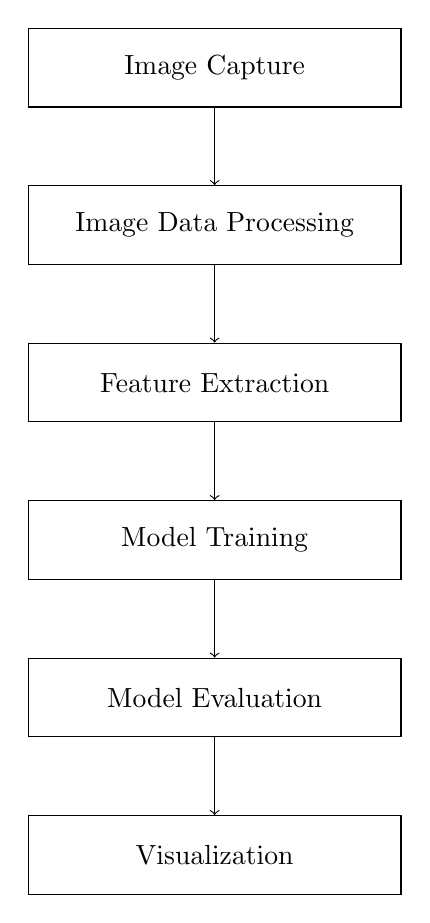
\begin{tikzpicture}[node distance=2cm, auto]
		% Node style
		\tikzstyle{block} = [rectangle, draw=black, text width=4.5cm, text centered, minimum height=1cm]
		
		% Nodes
		\node[block] (capture) {Image Capture};
		\node[block, below of=capture] (processing) {Image Data Processing};
		\node[block, below of=processing] (extraction) {Feature Extraction};
		\node[block, below of=extraction] (training) {Model Training};
		\node[block, below of=training] (evaluation) {Model Evaluation};
		\node[block, below of=evaluation] (visualization) {Visualization};
		
		% Arrows
		\draw[->] (capture) -- (processing);
		\draw[->] (processing) -- (extraction);
		\draw[->] (extraction) -- (training);
		\draw[->] (training) -- (evaluation);
		\draw[->] (evaluation) -- (visualization);
	\end{tikzpicture}
	\caption{ML Pipeline for Face Detection Evaluation Workflow}
	\label{FaceDetectionEvaluation}
\end{figure}



\subsection{Application}
The evaluation was applied to ensure robust model performance at each stage includes:
\begin{enumerate}
	\item \textbf{Image Capture}: Images captured by Vision Shield were tested for quality consistency under varied conditions.
	\item \textbf{Image Data Processing}: Validating the impact of preprocessing steps such as resizing, resolution check and augumentation.
	\item \textbf{Feature Extraction}: Ensuring the features extracted were meaningful and consistent across samples.
	\item \textbf{Evaluation Results}: Evaluating the machine learning model's performance using metrics such as accuracy, precision, recall, F1 score, and inference time
	\item \textbf{Model Testing}: Deploying the model in real-time with the Vision Shield Camera to test its performance to environmental changes.
\end{enumerate}

\subsection{Result}
Results from the evaluation phase, refer table ~\ref{tab:metrics}, figure ~\ref{EvaluationResults} include:
\begin{enumerate}
	\item \textbf{Accuracy}: The overall correctness of face detections.
	\item \textbf{Precision}: Proportion of true positive detections among all detections.
	\item \textbf{Recall}: Proportion of true positive detections among actual faces in the dataset.
	\item \textbf{F1 Score}: Balances precision and recall for an overall performance metric.
	\item \textbf{Inference Time}: Time taken for the model to process and predict for a single image.
\end{enumerate}

\begin{table}[h!]
	\centering
	\begin{tabular}{|l|c|}
		\hline
		\textbf{Metric}        & \textbf{Value} \\ \hline
		Accuracy               & 85.2\%         \\ \hline
		Precision              & 90\%           \\ \hline
		Recall                 & 85\%           \\ \hline
		F1 Score               & 84\%           \\ \hline
		Inference Time         & 1798ms         \\ \hline
	\end{tabular}
	\caption{Performance Metrics}
	\label{tab:metrics}
\end{table}

\begin{figure}
	\begin{center}
		\includegraphics[width=0.7\linewidth]{Images/EdgeImpulse/Interpretation.png}
		\caption{Model Evaluaiton Metrics}
		\label{EvaluationResults}
	\end{center}
\end{figure}

\section{Validation}
\subsection{Concept}
General validation ensures that the face detection system performs consistently and reliably across diverse conditions, including different lighting scenarios, facial orientations and environmental challenges. 

\subsection{Ideas}
\subsubsection{Cross-Validation}
\textbf{Purpose}: Ensure the model performs consistently across different data splits.
\\
\textbf{Method}: Dividing the dataset into several folds, iteratively train on some while validating on others and average the results.

\subsubsection{Real-Time Testing}
\textbf{Purpose}: Assess the model's functionality and robustness in real-world scenarios.
\\\textbf{Method}: Deploy the model on the Portenta H7 along with the Vision Shield Camera and test it under various lighting conditions, angles and environment.

\subsubsection{User Feedback:}
\textbf{Purpose}: To gather insights from users to identify any user issues and pinpoint areas for improvement in the face detection model.

\textbf{Method}: Deploy the model in live settings and collect feedback on detection accuracy, speed and usability.

\subsection{Conclusion}
By performing cross-validation, real-time testing and user feedbacks, we confirmed that the model achieves its goals of accurate and efficient face detection. These validation make sure that the system works well technically and is practical enough to be useful in everyday situations.

\subsection{Future Enhancements}
While the project has achieved significant success, there are still several opportunities for further enhancements and exploration, particularly in leveraging advanced communication methods like LoRa for remote access management and real-time monitoring.

\subsubsection{LoRa-Based Communication for Prediction Data}

The Portenta Vision Shield features built-in LoRa (Long Range) capabilities, offering a low-power, long-range wireless communication method. Future work could involve utilizing LoRa to transmit recognized face data to a remote server, enabling centralized monitoring and decision-making. This would be particularly valuable for applications in smart access control, security systems, and IoT-based facility management.

To implement LoRa communication efficiently, different approaches can be considered:

\begin{itemize}
	\item \textbf{LoRa Peer-to-Peer Communication:} This method allows direct data transmission between two devices without requiring additional infrastructure. This could be used to send face recognition results directly from the Portenta Vision Shield to a local receiver or security system. (Refer ~\ref{P2P})
	
	\item \textbf{LoRaWAN (LoRa Wide Area Network):} LoRaWAN enables data transmission over a broader network, allowing face recognition results to be sent to cloud-based systems or remote monitoring platforms. This would be ideal for large-scale security applications where multiple access points need to be synchronized in real-time. (Refer ~\ref{LORAWAN})
\end{itemize}


\chapter{Application Deployment}

\section{Description}
Model deployment is the process of integrating the trained face recognition model into a functional environment to perform real-time image recognition and transmission. This involves setting up the hardware, ensuring compatibility between components, and implementing the necessary software for smooth operation. The deployment is guided by the knowledge discovery in databases (KDD) process to ensure an efficient transition from development to application. \cite{IEEE:1997}

\section{Deployment Architecture}

The deployment architecture consists of three primary components: the Edge Device (Arduino Portenta H7), LoRa Communication Network, and the Centralized System for result processing and storage. Below is a breakdown of each component and their interactions:

\subsection{Edge Device (Arduino Portenta H7 + Vision Shield)}
The Edge Device is responsible for capturing images and processing them through the face recognition model. The steps involved are:

\begin{itemize}
	\item \textbf{Face Recognition Model}: The core model (converted to TensorFlow Lite) runs on the Portenta H7 microcontroller. It processes images captured by the Vision Shield.
	\item \textbf{Image Capture and Preprocessing}: The Vision Shield captures images and preprocesses them to meet the input requirements of the face recognition model.
	\item \textbf{Inference}: The preprocessed image is fed into the model for real-time face recognition.
	\item \textbf{Model Output}: The output (e.g., recognition result, identified face) is generated and prepared for transmission.
\end{itemize}

\begin{comment}
\subsection{LoRa Communication Network}
The LoRa communication network enables the wireless transmission of the face recognition results or image data. The components involved are:

\begin{itemize}
	\item \textbf{LoRa Transmitter}: The Portenta H7 communicates via a LoRa transceiver to wirelessly send the recognition results or image data.

	\item \textbf{Data Transmission}: Data is transmitted in small packets over long distances, optimized for low-power and low-bandwidth environments.
\end{itemize}

\subsection{Centralized System (Server or Cloud)}
The centralized system receives, processes and stores the transmitted data. The components involved are:

\begin{itemize}
	\item \textbf{Receiving Data}: The remote system (local server or cloud-based server) receives the transmitted data from the LoRa network.
	\item \textbf{Data Processing \& Storage}: The received results (face recognition data, image data) are processed further if needed and stored in a database for later analysis, reporting, or decision-making.
	\item \textbf{Real-Time Monitoring}: The system continuously monitors the deployed devices for performance, battery status, and model accuracy, ensuring that any issues can be addressed immediately.
\end{itemize}
\end{comment}

\section{Flow Chart of Each Step in the Deployment}

	\begin{figure}[h!]
	\centering
	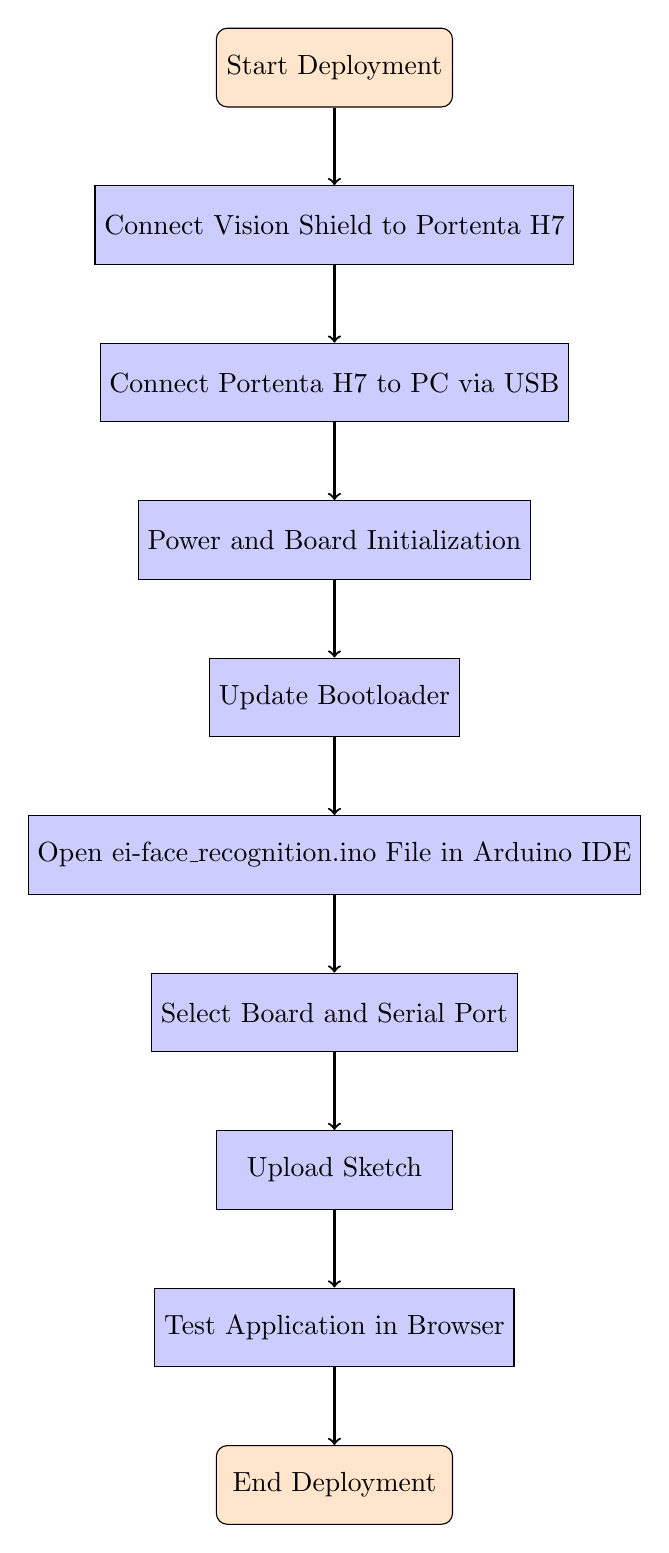
\begin{tikzpicture}[node distance=2cm, every node/.style={align=center}]
		
	% Nodes
	\node (start) [rectangle, minimum width=3cm, minimum height=1cm, text centered, draw=black, fill=orange!20, rounded corners] {Start Deployment};
	\node (load) [rectangle, minimum width=3cm, minimum height=1cm, text centered, draw=black, fill=blue!20, below of=start] {Connect Vision Shield to Portenta H7};
	\node (configure) [rectangle, minimum width=3cm, minimum height=1cm, text centered, draw=black, fill=blue!20, below of=load] {Connect Portenta H7 to PC via USB};
	\node (capture) [rectangle, minimum width=3cm, minimum height=1cm, text centered, draw=black, fill=blue!20, below of=configure] { Power and Board Initialization};
	\node (preprocess) [rectangle, minimum width=3cm, minimum height=1cm, text centered, draw=black, fill=blue!20, below of=capture] {Update Bootloader};
	\node (inference) [rectangle, minimum width=3cm, minimum height=1cm, text centered, draw=black, fill=blue!20, below of=preprocess] {Open ei-face\_recognition.ino File in Arduino IDE};
	\node (transmit) [rectangle, minimum width=3cm, minimum height=1cm, text centered, draw=black, fill=blue!20, below of=inference] {Select Board and Serial Port};
	\node (monitoring) [rectangle, minimum width=3cm, minimum height=1cm, text centered, draw=black, fill=blue!20, below of=transmit] {Upload Sketch};
	\node (updates) [rectangle, minimum width=3cm, minimum height=1cm, text centered, draw=black, fill=blue!20, below of=monitoring] {Launch Command Prompt};
	\node (updates) [rectangle, minimum width=3cm, minimum height=1cm, text centered, draw=black, fill=blue!20, below of=monitoring] {Test Application in Browser};
	\node (end) [rectangle, minimum width=3cm, minimum height=1cm, text centered, draw=black, fill=orange!20, rounded corners, below of=updates] {End Deployment};
	
		
		% Arrows
		\draw[thick,->] (start) -- (load);
		\draw[thick,->] (load) -- (configure);
		\draw[thick,->] (configure) -- (capture);
		\draw[thick,->] (capture) -- (preprocess);
		\draw[thick,->] (preprocess) -- (inference);
		\draw[thick,->] (inference) -- (transmit);
		\draw[thick,->] (transmit) -- (monitoring);
		\draw[thick,->] (monitoring) -- (updates);
		\draw[thick,->] (updates) -- (end);
		
	\end{tikzpicture}
	\caption{Deployment Process Flowchart}
	\label{fig:deployment-flow}
\end{figure}


\section{ML Pipeline}

\tikzstyle{process} = [rectangle, minimum width=0.2cm, minimum height=0.1cm, text centered, draw=black, fill=blue!20]
\tikzstyle{yellowprocess} = [rectangle, minimum width=0.2cm, minimum height=0.1cm, text centered, draw=black, fill=orange!20]
\tikzstyle{arrow} = [thick,->,>=stealth]

	\begin{figure}[h!]
	\centering
	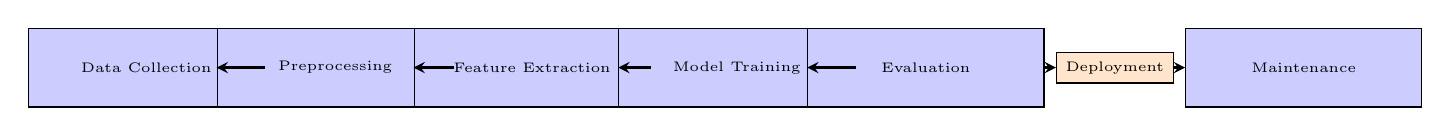
\begin{tikzpicture}[node distance=2.4cm, 
		every node/.style={align=center}] 
		
		% Nodes
		\node (block1) [process] {\tiny Data Collection};
		\node (block2) [process, right of=block1] {\tiny Preprocessing};
		\node (block3) [process, right of=block2, node distance=2.5cm] {\tiny Feature Extraction};  % Reduced distance
		\node (block4) [process, right of=block3, node distance=2.6cm] {\tiny Model Training};  % Reduced distance
		\node (block5) [process, right of=block4] {\tiny Evaluation};
		\node (block6) [yellowprocess, right of=block5] {\tiny Deployment};  % Changed color to yellow
		\node (block7) [process, right of=block6] {\tiny Maintenance};
		
		% Arrows
		\draw [arrow] (block1) -- (block2);
		\draw [arrow] (block2) -- (block3);
		\draw [arrow] (block3) -- (block4);
		\draw [arrow] (block4) -- (block5);
		\draw [arrow] (block5) -- (block6);
		\draw [arrow] (block6) -- (block7);
		
	\end{tikzpicture}
	\caption{Machine Learning Pipeline}
	\label{fig:MLPipeline}
\end{figure}

The machine learning pipeline in the deployment process includes the following steps:

\begin{itemize}
	\item \textbf{Data Collection:} Capturing images using the Arduino Portenta H7 with Vision Shield.
	\item \textbf{Preprocessing:} Resizing, converting to grayscale, and cleaning images.
	\item \textbf{Feature Extraction:} Extracting relevant features from the preprocessed images.
	\item \textbf{Model Training:} Training the machine learning model with the extracted features.
	\item \textbf{Evaluation:} Assessing the model’s performance and accuracy.
	\item \textbf{Deployment:} Implementing the model into the Arduino Portenta H7 with Vision Shield.
	\item \textbf{Maintenance:} Regularly updating the model and ensuring its continuous performance.
\end{itemize}

\section{Process}

The deployment process for the face recognition application using the Arduino Portenta H7, Vision Shield, and LoRa device involves multiple detailed steps to ensure seamless functionality. Below is a comprehensive guide:

\subsection{Connect the Vision Shield to the Arduino Portenta H7}

\textbf{Hardware Connection:}  
\begin{itemize}[leftmargin=1.5cm]
	\item Attach the Vision Shield to the Arduino Portenta H7 via the designated connectors.
	\item Ensure the Vision Shield is firmly seated to avoid loose connections.
	\item Verify the Vision Shield’s orientation to prevent incorrect installation.
\end{itemize}

\subsection{Connect the Arduino Portenta H7 to the System}

\textbf{USB Connection:}  
\begin{itemize}[leftmargin=1.5cm]
	\item Connect the Portenta H7 to your computer using a USB-C cable.
	\item Ensure the cable is in good condition to avoid connection interruptions.
	\item Confirm the connection by checking for a detected COM port in the Arduino IDE or using \texttt{ls /dev/tty*} in Linux/Mac.
\end{itemize}

\subsection{Check Power Supply and Board Initialization}

\textbf{Power Supply:}  
\begin{itemize}[leftmargin=1.5cm]
	\item Ensure the Portenta H7 receives a stable power supply (5V via USB-C or external battery).
	
	\begin{figure}
		\begin{center}
			
			\includegraphics[width=0.4\linewidth]{images/ArduinoIDE/ArduinoPortentaH7Connectedtoalaptop.png}
			\captionof{figure}{Arduino PortentaH7 Connected to a Laptop}
			\label{Arduino PortentaH7 Connected to a Laptop1}
		\end{center}
		
	\end{figure}
	
	\item Check the onboard LED to confirm power delivery  as shown in the Figure \ref{Arduino PortentaH7 Connected to a Laptop1}.
\end{itemize}

\textbf{Board Initialization:}  
\begin{itemize}[leftmargin=1.5cm]
	\item Open the Arduino IDE and launch the Serial Monitor.
	\item Set the baud rate to 115200 and verify the initialization messages to ensure the board starts correctly.
\end{itemize}

\begin{comment}
\subsection{Configure LoRa Communication}

\textbf{Hardware and Frequency Setup:}  
\begin{itemize}[leftmargin=1.5cm]
	\item Attach the LoRa module to the Portenta H7 via SPI pins.
	\item Configure LoRa frequency settings (e.g., 868 MHz for Europe or 915 MHz for the USA) within the code.
\end{itemize}

\textbf{Test LoRa Communication:}  
\begin{itemize}[leftmargin=1.5cm]
	\item Use a basic transmit/receive test sketch to verify the connection between the LoRa module and the Portenta H7.
\end{itemize}
\end{comment}

\subsection{Load the Face Recognition Sketch}

\textbf{Open Project:}  
\begin{itemize}[leftmargin=1.5cm]
	\item Launch the Arduino IDE and open the file \texttt{.ino} for the face recognition project.
	\item Ensure the sketch includes:
	\begin{itemize}
		\item Image capture and preprocessing from the Vision Shield.
	\end{itemize}
\end{itemize}

\textbf{Board and Port Selection:}  
\begin{itemize}[leftmargin=1.5cm]
	\item Select the correct board (Arduino Portenta H7) and corresponding serial port from the Arduino IDE.
\end{itemize}

\subsection{Compile and Upload the Sketch}

\textbf{Compilation:}  
\begin{itemize}[leftmargin=1.5cm]
	\item Click on the ‘Verify’ button to compile the code and check for errors.
\end{itemize}

\textbf{Upload:}  
\begin{itemize}[leftmargin=1.5cm]
	\item Click the ‘Upload’ button to flash the sketch onto the Portenta H7.
	\item Monitor the Serial Monitor to confirm successful upload and initialization.
\end{itemize}

\subsection{Run and Test the Model}

\textbf{Launch Impulse Runner:}  
\begin{itemize}[leftmargin=1.5cm]
	\item Open a terminal and run the Edge Impulse command to initiate the model as shown in the figure ~\ref{inference}:  
	 \\ \SHELL{edge-impulse-run-impulse}  
	\item This will execute the face recognition inference on the Portenta H7.
\end{itemize}

\textbf{Debug Mode and Real-Time Monitoring:}  
\begin{itemize}[leftmargin=1.5cm]
	\item Enable debug mode for real-time inference monitoring by running the below command in the terminal as shown in the figure ~\ref{debug}:
	\\ \SHELL{edge-impulse-run-impulse --debug} 
	\item Open the provided URL to visualize the live camera feed and check predictions in real-time.
\end{itemize}

\begin{figure}
	\begin{center}
		\includegraphics[width=0.7\linewidth]{Images/EdgeImpulse/run_impulse.png}
		\caption{Running the inference}
		\label{inference}
	\end{center}
\end{figure}

\begin{figure}
	\begin{center}
		\includegraphics[width=0.7\linewidth]{Images/EdgeImpulse/impulse_debug.png}
		\caption{Debug Mode}
		\label{debug}
	\end{center}
\end{figure}

\begin{comment}

\subsection{Verify LoRa Transmission}

\textbf{Transmit Inference Results:}  
\begin{itemize}[leftmargin=1.5cm]
	\item Ensure the inference results (e.g., recognized face labels) are transmitted via LoRa.
	\item Use a receiving LoRa device or gateway to verify successful transmission and reception.
\end{itemize}
\end{comment}


\chapter{Monitoring and Maintenance}
This chapter outlines the strategies for monitoring the deployed face detection model and maintaining its performance over time.

\section{Idea}
The concept of monitoring and maintenance of the face detection system is designed to allow dynamic updates such as adding or removing individuals from the dataset by incorporating new data, updating the pipeline and performing regular checks.

\begin{figure}
	\begin{center}
		\includegraphics[width=0.7\linewidth]{Images/EdgeImpulse/RetrainModel.png}
		\caption{Model Retraining}
		\label{RetrainModel}
	\end{center}
\end{figure}

\section{Plan/Description}
The concept for the face detection system is focused on dynamic dataset management includes setting up a system for regular model evaluation, data collection, and retraining and system adaptability. The primary goals are:

\begin{enumerate}
	\item \textbf{Dataset Updates}: Add new users by collecting and processing their face data or remove users to revoke access, ensuring the dataset stays current.  
	\item \textbf{Model Retraining}: Retrain the model to reflect the updated dataset, to maintain accuracy and reliability.  
	\item \textbf{Evaluate the Retrained Model}: Assess the updated model’s performance on metrics like accuracy, precision, and recall to ensure quality.  
	\item \textbf{Deploy the Model}: Deploy the system with the retrained model for consistent real-time performance.  
\end{enumerate}

\section{Updating new Data}
The dataset can be updated using Edge impulse data collection tool. This involves capturing multiple face images for new users under various conditions using Vision Shield Camera or removing the existing datasets in the Edge Impulse Dataset explorer.

New face data is added when new users need access. This data is then used for retraining the machine learning model.

\section{Data updating in the ML Pipeline}
Data updation in the ML Pipeline includes the following steps:
\begin{enumerate}
	\item Add the new faceset data or remove the existing faceset in the Edge Impulse data collection tool
	\item Preprocess the updated data to align with existing datasets.
	\item Retraining the model with the updated dataset to incorporate changes
\end{enumerate}

\section{Checks}
To ensure the system remains reliable:
\begin{enumerate}
	\item \textbf{Performance Metrics}: Regularly monitor accuracy, precision, recall, and inference times.
	\item \textbf{Dataset Integrity}: Review the dataset to avoid duplicates or inconsistencies.
	\item \textbf{Testing}: Perform routine testing in real-world conditions to identify potential issues early.
\end{enumerate}

\section{Privacy}
To ensure privacy in the face access system:
\begin{enumerate}
	\item \textbf{Anonymization}: All collected data is anonymized to protect user identity.
	\item \textbf{Secure Access Control}: Data is securely stored, and access is restricted to authorized personnel through strict permissions.
\end{enumerate}

\section{Robustness}
To maintain the system's effectiveness:
\begin{enumerate}
	\item Test the model under varying conditions such as lighting changes or occlusions.
	\item Redundant systems to ensure data collection and model evaluation continue unin
	terrupted.
	\item Regularly update the model to adapt to changing user requirements and scenarios.
\end{enumerate}

\begin{figure}[h]
	\centering
	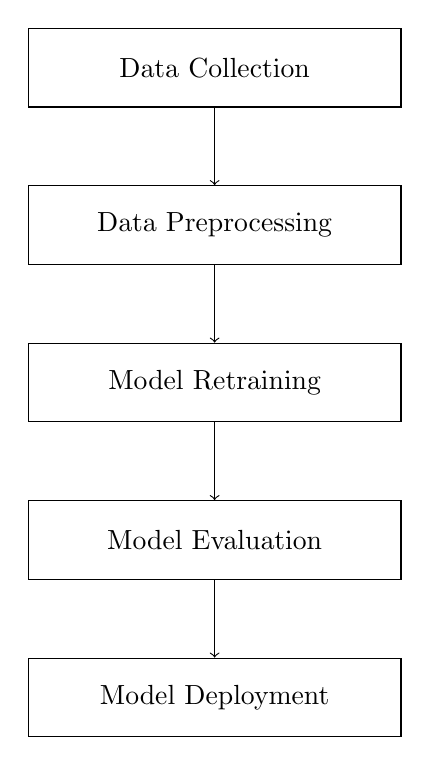
\begin{tikzpicture}[node distance=2cm, auto]
		% Node style
		\tikzstyle{block} = [rectangle, draw=black, text width=4.5cm, text centered, minimum height=1cm]
		
		% Nodes
		\node[block] (collection) {Data Collection};
		\node[block, below of=collection] (preprocessing) {Data Preprocessing};
		\node[block, below of=preprocessing] (retraining) {Model Retraining};
		\node[block, below of=retraining] (evaluation) {Model Evaluation};
		\node[block, below of=evaluation] (deployment) {Model Deployment};
		
		% Arrows
		\draw[->] (collection) -- (preprocessing);
		\draw[->] (preprocessing) -- (retraining);
		\draw[->] (retraining) -- (evaluation);
		\draw[->] (evaluation) -- (deployment);
	\end{tikzpicture}
	\caption{Process Workflow for Face Access System Monitoring}
	\label{FaceAccessMonitoring}
\end{figure}


\section{Process}

The overall workflow for the face access system includes the following steps, refer figure ~\ref{FaceAccessMonitoring}:

\begin{enumerate}
	\item \textbf{Data Collection:} Capture new face images from the deployed system for adding new facesets.
	\item \textbf{Data Preprocessing:} Clean and preprocess the new data to ensure it aligns with the model’s input requirements.
	\item \textbf{Model Retraining:} Retrain the model using the updated dataset to incorporate new faces and improve performance.
	\item \textbf{Model Evaluation:} Evaluate the performance of the retrained model using metrics like accuracy, precision, and recall to ensure it meets the required standards.
	\item \textbf{Model Deployment:} Deploy the updated model back into the system, ensuring that it operates smoothly with the updated data.
\end{enumerate}


\begin{comment}

\chapter{Face recognition using Edge Impulse}
\section{Introduction}
In this chapter, we are going to look at how to train a face detection model and the steps required in training and deploying a model with Edge Impulse platform using Portenta H7 and Vision Shield.

\section{Procedure}
Edge Impulse offers a cloud-based system for data collection, neural network design, model training, testing and deployment, streamlining the end-to-end machine learning workflow for edge devices. The workflow for the overall process is shown in the figure ~\ref{fig:face_recognition_flow}

\tikzstyle{startstop} = [ellipse, minimum width=3cm, minimum height=1cm, text centered, draw=black, fill=gray!30]
\tikzstyle{process} = [rectangle, minimum width=3cm, minimum height=1cm, text centered, draw=black, fill=blue!20]
\tikzstyle{edge} = [rectangle, minimum width=3cm, minimum height=1cm, text centered, draw=black, fill=orange!20]
\tikzstyle{decision} = [diamond, minimum width=3cm, minimum height=1cm, text centered, draw=black, fill=blue!20]
\tikzstyle{arrow} = [thick,->,>=stealth]


\begin{figure}[h!]
	\centering
\begin{tikzpicture}[node distance=2cm]
	
	% Nodes
	\node (start) [startstop] {Input Image};
	\node (label) [process, below of=start] {Image Labelling};
	\node (preprocess) [process, below of=label] {Image Pre-processing};
	\node (feature) [process, below of=preprocess] {Feature Extraction};
	\node (train) [process, below of=feature] {Train the model (CNN)};
	\node (decision) [decision, below of=train, yshift=-1.2cm] {Output Predicted};
	\node (save) [process, below of=decision, yshift=-1.2cm] {Save model into tflite format};
	\node (deploy) [edge, below of=save] {Deploy to Arduino Portenta H7};
	\node (detect) [edge, below of=deploy] {Detect face using vision shield};
	
	% Arrows
	\draw [arrow] (start) -- (label);
	\draw [arrow] (label) -- (preprocess);
	\draw [arrow] (preprocess) -- (feature);
	\draw [arrow] (feature) -- (train);
	\draw [arrow] (train) -- (decision);
	\draw [arrow] (decision) -- node[anchor=west] {Yes} (save);
	\draw [arrow] (save) -- (deploy);
	\draw [arrow] (deploy) -- (detect);
	\draw [arrow] (decision.east) -- node[anchor=south] {No} ++(1,0) |- (train);
	
\end{tikzpicture}
\caption{Flowchart for overall process}
\label{fig:face_recognition_flow}
\end{figure}

\section{Database}
To train a machine learning model for face recognition we first need to create a database
of images consisting of faces. We can create it by capturing the images using the Vision Shield Camera.
\subsection{Database Preparation}
In this project, we are using our own database for model training and testing. We are going to use three distinct dataset of faces and labeled them into Vatsal, Manoj and Vijay. To train the model we need sufficient images under different conditions (lightings, angle) for better performance. So, we are using 50-70 images per dataset and the dimensions of the images in the dataset is 160 x 120 pixels. In the figure ~\ref{Dataset}, we can see the sample images used in the project database.

\begin{figure}
	\begin{center}
		\includegraphics[width=0.7\linewidth]{Images/EdgeImpulse/Dataset.png}
		\caption{Sample Dataset}
		\label{Dataset}
	\end{center}
\end{figure}

\subsection{Uploading the dataset in the Edge Impulse}
Firstly, we need to login in the Edge Impulse portal \href{https://studio.edgeimpulse.com/}{EdgeImpulse} and create a project named Face\_recognition. In order to upload our image dataset, we need to go to the Edge Impulse dashboard and click on acquire data and select upload data. For uploading the dataset of images captured by Arduino Vision Shield, we need to connect it to the Edge Impulse Platform. This is described in the next section.

\section{Connecting the Arduino Portenta H7 with Edge Impulse}
In order to take pictures from the vision shield, we need to connect our device to the
Edge Impulse portal and then start taking pictures. To do this, we need to install the
following software.
\begin{itemize}
	\item \textbf{Arduino CLI}: We need to download the Arduino CLI from the website \href{https://arduino.github.io/arduino-cli/1.0/installation/}{ArduinoCLI-Installation} and extract the following Zip file named \FILE{arduino-cli\_1.0.4\_Windows\_64bit.zip}.Then we need to add the extracted file path which is \PATH{C:/Program Files/Arduino CLI} in the Environment Variables lists on our computer. After adding the path, we need to open command prompt and type \SHELL{Arduino-cli} and press enter to install it. After the installation is done, type \SHELL{arduino-cli board list} in the command prompt. It displays the connected device as Arduino Portenta H7 with Port number and type as shown in the figure ~\ref{boardlistCmd}
	\begin{figure}
		\begin{center}
			\includegraphics[width=0.7\linewidth]{Images/EdgeImpulse/Nodejs.png}
			\caption{Arduino CLI Board List command}
			\label{boardlistCmd}
		\end{center}
	\end{figure}
	
	\item \textbf{Edge Impulse CLI} : We first need to install Python 3 and download Node.js version latest version from the website \href{https://nodejs.org/en/}{Node.js}. The downloaded Windows installer file is named as \FILE{node-v20.17.0-x64.msi}. Then we need to begin installing by opening this Windows installer file. Click on install, ensuring to include all the necessary tools during installation by checking the check box as shown in the figure ~\ref{NodejsInstallation2} and the installed path is \PATH{C:/ProgramData/Microsoft/Windows/\\StartMenu/Programs/Node.js} After the installation is done we need to open the command prompt and type \SHELL{npm install-g edge-impulse-cli–force} to install it. \cite{edgeimpulse_cli:2024}
	
	\begin{figure}
		\begin{center}
			\includegraphics[width=0.7\linewidth]{Images/EdgeImpulse/Nodejs.png}
			\caption{Node.js Installation}
			\label{NodejsInstallation2}
		\end{center}
	\end{figure}
	
\end{itemize}

\section{Data Labeling}
Now that we need to label the data for uploading dataset. To do this, go to the Dashboard of the project and choose the Labeling method. Select 'One Label per data item' since in face recognition, each image typically contains single face and we are classifying the entire image as belonging to a specific person as shown in the figure ~\ref{DataLabel}. Then while uploading data, give label name for the three distinct image to differentiate.

\begin{figure}
	\begin{center}
		\includegraphics[width=0.7\linewidth]{Images/EdgeImpulse/DataLabel.png}
		\caption{Data Labeling Method}
		\label{DataLabel}
	\end{center}
\end{figure}

\section{Data Transformation}
\subsection{Designing the Impulse}
For designing the impulse, click on Impulse design and then set the image width
and height to 160X160 pixel and Resize mode to 'Fit longest', because it offers enough resolution to capture important facial features while being small enough to run efficiently on the Portenta H7. We can reduce the pixel further if we need faster inference. Then in the pre-processing block, select the 'Image'. The image pre-processing block takes input image and can optionally convert it into grayscale and then turns the data into a features array. Then we need to add a learning block and select 'Transfer Learning (images)'. Finally, save the impulse as shown in the figure ~\ref{Impulse}.

 \begin{figure}
 	\begin{center}
 		\includegraphics[width=0.7\linewidth]{Images/EdgeImpulse/ImpulseDesign.png}
 		\caption{Impulse Design}
 		\label{Impulse}
 	\end{center}
 \end{figure}
 
 \subsection{Configuring the Image processing block}
 To configure the processing block, click Images in the menu on the left. This will show us the raw data on top of the screen and the results of the processing step on the right.  we can also use the options to switch between 'RGB' and 'Grayscale' mode. We then click on save parameters as shown in figure ~\ref{Feature}.
 
 \begin{figure}
 	\begin{center}
 		\includegraphics[width=0.7\linewidth]{Images/EdgeImpulse/FeatureExtract.png}
 		\caption{Save Parameters}
 		\label{Feature}
 	\end{center}
 \end{figure}

Then click on generate features option on the top and then click on generate features. In the figure ~\ref{GenerateFeature}, we can see that features generated from the dataset of images consisting of three distinct faces with distinguishable data points.

\begin{figure}
	\begin{center}
		\includegraphics[width=0.7\linewidth]{Images/EdgeImpulse/GenerateFeatures.png}
		\caption{Generate Features}
		\label{GenerateFeature}
	\end{center}
\end{figure}

\section{Data Training}
\subsection{Configuring the transfer training model:}
Here we are using transfer learning block because it is easier to use a pre-trained model by only retaining the upper layers of a neural network and then we can train the model in a short time. To configure the transfer learning model, click on transfer learning on the left. Here, we can set the learning rate, in our case we have set it to 0.0005 and the number of training cycles to 25. Then we select the base model, here we have selected as MobileNetV2 and then click on Save and Train. After the training process is completed we can see from the figure ~\ref{ModelTrain}, accuracy of 93.2\% is achieved.

\begin{figure}
	\begin{center}
		\includegraphics[width=0.7\linewidth]{Images/EdgeImpulse/TransferLearning.png}
		\caption{Model Training}
		\label{ModelTrain}
	\end{center}
\end{figure}

\section{Testing the Model}
In order to test the model, we need to click on the option Model testing and then click on classify all. Here, the dataset images were automatically divided into training and testing images. Here, the model divided the input images into training images consisting of 129 images and testing consisting of 38 images. The testing images are then used to check how well the model performs. As we can see from the figure ~\ref{ModelTest}, that the model achieved 94.59\% accuracy.

\begin{figure}
	\begin{center}
		\includegraphics[width=0.7\linewidth]{Images/EdgeImpulse/ModelTest.png}
		\caption{Testing the Model}
		\label{ModelTest}
	\end{center}
\end{figure}

We can also do the live classification and recognize face in real time using the vision shield. Click on the Live classification option in the menu and connect our Portenta H7 device with the Edge Impulse by selecting the device on the drop-down option. Then as soon as it is connected we can see the camera stream from vision shield. Here we have tested the model by focusing on face and as we can see from the figure ~\ref{LiveClassify}, that it gives the output as face with 0.89 value which is a pretty good prediction.

\begin{figure}
	\begin{center}
		\includegraphics[width=0.7\linewidth]{Images/EdgeImpulse/LiveClassify.png}
		\caption{Live Classification using Vision Shield Camera}
		\label{LiveClassify}
	\end{center}
\end{figure}

\section{Model Deployment}
In order to perform deployment, click on the option Deployment and search for Arduino Library as shown in the figure ~\ref{ModelDeployment}, to build the model for Arduino library. Select the Model Optimization as Quantized (int8) to increase on-device performance and faster inference and click Build.

\begin{figure}
	\begin{center}
		\includegraphics[width=0.7\linewidth]{Images/EdgeImpulse/ModelDeployment.png}
		\caption{Model Deployment}
		\label{ModelDeployment}
	\end{center}
\end{figure}

\section{Running the inference and testing}
Once the building the model is completed, it is downloaded as zip file called \FILE{ei-face\_recognition-arduino-1.0.13.zip}. Now open Arduino IDE and add this downloaded library through the Arduino IDE via \PATH{Sketch > Include Library > Add .ZIP Library} as shown in the figure ~\ref{ZIP}. Then go to \PATH{Files > Examples > Face\_recognition\_inferencing > portenta\_h7 > portenta\_h7\_camera} as shown in the figure ~\ref{FaceRecognition} to get the code for face recognition using edge impulse with the model developed. 

\begin{figure}
	\begin{center}
		\includegraphics[width=0.7\linewidth]{Images/EdgeImpulse/AddZIP.png}
		\caption{Adding the downloaded library through Arduino IDE}
		\label{ZIP}
	\end{center}
\end{figure}

\begin{figure}
	\begin{center}
		\includegraphics[width=0.7\linewidth]{Images/EdgeImpulse/FaceRecognition.png}
		\caption{Program code for Face Recognition}
		\label{FaceRecognition}
	\end{center}
\end{figure}

Before uploading the model, connect Arduino Portenta H7 along with the Vision Shield to the PC. Check the Board manager configurations are properly set by going to \PATH{Tools > Board} and select Arduino Portenta H7 (M7 core) and check the COM port is recognizable in \PATH{Tools > Port}. Then compile and upload the code in Arduino IDE.
Once the code is uploaded to the Arduino Portenta H7, run the inference by using the command \SHELL{edge-impulse-run-impulse} in the command prompt as shown in the figure. Then to visualise the result in the web browser, run the command \SHELL{edge-impulse-run-impulse --debug} and we get the local IP address to forcast the result as shown in the figures ~\ref{Vijay} and ~\ref{Uncetrain} between trained images and uncertain image.

\begin{figure}
	\begin{center}
		\includegraphics[width=0.7\linewidth]{Images/EdgeImpulse/Vijay.png}
		\caption{Predicted face image}
		\label{Vijay}
	\end{center}
\end{figure}
\begin{figure}
	\begin{center}
		\includegraphics[width=0.7\linewidth]{Images/EdgeImpulse/Uncertain.png}
		\caption{Uncertain face image}
		\label{Uncetrain}
	\end{center}
\end{figure}

\chapter{Updating the face access}
In this section, we are going to add and remove a face profile using Edge Impulse API. This involves setting up an automated pipeline where face images are dynamically uploaded to Edge Impulse, retrained, and then the new model is automatically deployed to your Arduino Portenta H7.

\section{Set up Edge Impulse API Access}
To start with, we need a API access to our Edge Impulse Project. So, API helps us to upload new datasets programmatically, retrain the model and finally to deploy in Arduino Portenta H7.
Click the project Dashboard in the Edge Impulse Studio. Select the Keys option on the top of the taskbar. Now, copy the API key available in the API Key section, which will be used for all API requests as shown in the figure ~\ref{API}.

\begin{figure}
	\begin{center}
		\includegraphics[width=0.7\linewidth]{Images/EdgeImpulse/API.png}
		\caption{API key}
		\label{API}
	\end{center}
\end{figure}

\section{Capturing and Uploading New Faces via API}
In this stage, we are going to see how to capture and upload the new face images into the Edge Impulse dataset, to whom we are going to give new access.

To capture the new images, we are using 50-70 images for the dataset and label them into Person4. In order to get better performance, we are using images under different conditions (lightnings, angle), as we did earlier and the dimensions of the images is 160 x 120 pixels. In the figure, we can see the sample images of the label used in the project.

\end{comment}